\begin{enumerate}

    % ==================================================================
    \item 35 kV 线路 \(l=30\ \mathrm{km}\)，\(r_1=0.2\ \Omega/\mathrm{km}\)，
          \(x_1=0.4\ \Omega/\mathrm{km}\)，\(P+jQ=8+j4\ \mathrm{MVA}\)，
          末端电压为 \(34\ \mathrm{kV}\)。求首端电压和功率损耗。

          \begin{solution}
              \begin{coursebox}
                  \textbf{来源：}第八章课件第 37 页“课程作业”第 1 题；电压降落公式见第 5、7 页，串联支路功率损耗公式见第 9 页，逐段推算法见第 13--14 页。

                  \smallskip
                  \textbf{思路：}同一端的 \(U_2\)、\(\tilde S_2\) 均已知，可直接从末端推算：先算线路串联损耗得 \(\tilde S_1\)，再由纵、横电压降得 \(U_1\)。题中未给 \(b_1\)，按短线路只计串联阻抗，且无需假设全网为额定电压。
              \end{coursebox}

              \stephead{（1）线路参数与功率损耗}

              线路总阻抗为
              \begin{equation*}
                  Z_L=(0.2+j0.4)\times30=6+j12\ \Omega.
              \end{equation*}

              由课件第 9 页的串联支路损耗公式，
              \begin{align*}
                  \Delta \tilde S_L
                   & =\frac{P_2^2+Q_2^2}{U_2^2}(R+jX)
                  =\frac{8^2+4^2}{34^2}(6+j12)                         \\
                   & =0.06920(6+j12)
                  =\boxed{0.415+j0.830\ \mathrm{MVA}}.
              \end{align*}

              因此首端功率为
              \begin{equation*}
                  \tilde S_1=\tilde S_2+\Delta \tilde S_L
                  =8+j4+0.415+j0.830
                  =\boxed{8.415+j4.830\ \mathrm{MVA}}.
              \end{equation*}

              \stephead{（2）首端电压}

              由课件第 5 页，电压降落的纵、横分量分别为
              \begin{align*}
                  \Delta U & =\frac{P_2R+Q_2X}{U_2}
                  =\frac{8\times6+4\times12}{34}
                  =2.824\ \mathrm{kV},                                  \\
                  \delta U & =\frac{P_2X-Q_2R}{U_2}
                  =\frac{8\times12-4\times6}{34}
                  =2.118\ \mathrm{kV}.
              \end{align*}

              若保留横分量，则
              \begin{equation*}
                  U_1=\sqrt{(U_2+\Delta U)^2+(\delta U)^2}
                  =\sqrt{(34+2.824)^2+2.118^2}
                  =\boxed{36.88\ \mathrm{kV}}.
              \end{equation*}

              首端电压超前末端电压
              \begin{equation*}
                  \theta=\arctan\frac{2.118}{36.824}
                  \approx 3.29^\circ.
              \end{equation*}

              若按课件第 7 页忽略横分量，则
              \begin{equation*}
                  U_1\approx U_2+\Delta U
                  =34+2.824
                  =\boxed{36.82\ \mathrm{kV}}.
              \end{equation*}

              \stephead{（3）结果}

              \begin{equation*}
                  \boxed{\tilde S_1\approx 8.42+j4.83\ \mathrm{MVA}},
                  \qquad
                  \boxed{U_1\approx 36.8\ \mathrm{kV}}.
              \end{equation*}

              线路有功损耗为 \(0.415\ \mathrm{MW}\)，无功损耗为
              \(0.830\ \mathrm{Mvar}\)，线损率约为
              \begin{equation*}
                  \frac{0.415}{8}\times100\%\approx 5.19\%.
              \end{equation*}

              按课件近似法取 \(36.82\ \mathrm{kV}\)；若保留横分量，则为
              \(36.88\angle3.29^\circ\ \mathrm{kV}\)，两者相差仅 \(0.06\ \mathrm{kV}\)。
          \end{solution}

    % ==================================================================
    \item 电力线路长 \(100\ \mathrm{km}\)，额定电压为 \(110\ \mathrm{kV}\)，末端接有一台容量为
          \(20\ \mathrm{MVA}\)、变比为 \(110/38.5\ \mathrm{kV}\) 的降压变压器。变压器低压侧负荷为
          \((15+j11.25)\ \mathrm{MVA}\)。正常运行时要求电压达 \(36\ \mathrm{kV}\)。试求线路始端母线应具备的功率和电压。

          线路采用 LGJ-120 导线，其单位长度参数为
          \begin{equation*}
              r_1=0.27\ \Omega/\mathrm{km},\quad
              x_1=0.412\ \Omega/\mathrm{km},\quad
              g_1=0,\quad
              b_1=2.76\times10^{-6}\ \mathrm{S/km}.
          \end{equation*}

          归算至 \(110\ \mathrm{kV}\) 侧的变压器参数为
          \begin{equation*}
              R_T=4.93\ \Omega,\quad
              X_T=63.5\ \Omega,\quad
              G_T=4.95\times10^{-6}\ \mathrm{S},\quad
              B_T=49.5\times10^{-6}\ \mathrm{S}.
          \end{equation*}

          \begin{figure}[H]
              \centering
              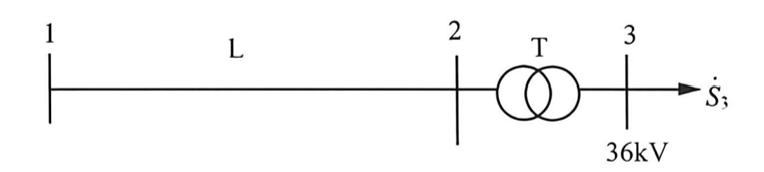
\includegraphics[width=0.68\textwidth]{problem2.png}
              \caption{第 2 题接线图（课件第 37 页）}
              \label{fig:problem2}
          \end{figure}

          \begin{solution}
              \begin{coursebox}
                  \textbf{来源：}第八章课件第 37 页第 2 题及接线图；逐段推算法见第 13--14 页，电压降落与功率损耗公式见第 5、7、9 页；变压器变比定义见第四章课件第 12 页。

                  \smallskip
                  \textbf{思路：}这是不同电压等级的辐射形开式网，按第 14 页“已知末端功率、电压”的方法从末端向首端推算：
                  \textcircled{1} 将 \(36\ \mathrm{kV}\) 按 \(110/38.5\) 归算到 \(110\ \mathrm{kV}\) 侧；
                  \textcircled{2} 变压器串联损耗和压降得 \(U_2\)；
                  \textcircled{3} 用 \(U_2\) 算变压器励磁和线路末端充电；
                  \textcircled{4} 线路串联损耗和压降得 \(U_1\)；
                  \textcircled{5} 用 \(U_1\) 算线路首端充电得 \(\tilde S_1\)。
                  关键是并联支路必须用所在节点的实际电压，不能全程用 \(110\ \mathrm{kV}\)。
              \end{coursebox}

              \stephead{（1）把低压侧电压归算到 110 kV 侧}

              变压器变比为 \(110/38.5\)，因此低压侧 \(36\ \mathrm{kV}\) 归算到高压侧为
              \begin{equation*}
                  U_3'=36\times\frac{110}{38.5}
                  =102.857\ \mathrm{kV}.
              \end{equation*}

              注意不能把 \(36\ \mathrm{kV}\) 直接当作高压侧电压，也不能用 \(110/36\) 作变比；归算时应使用变压器额定变比 \(110/38.5\)。

              \stephead{（2）线路和变压器参数}

              \begin{equation*}
                  R_L=27\ \Omega,\qquad
                  X_L=41.2\ \Omega,\qquad
                  B_L=2.76\times10^{-4}\ \mathrm{S}.
              \end{equation*}

              线路两端并联电纳各为 \(B_L/2=1.38\times10^{-4}\ \mathrm{S}\)。变压器参数为
              \begin{equation*}
                  Z_T=4.93+j63.5\ \Omega,\qquad
                  Y_T=(4.95+j49.5)\times10^{-6}\ \mathrm{S}.
              \end{equation*}

              按课件记法，\(B_T\) 取变压器励磁支路感性无功损耗对应的正值，因此励磁支路损耗写成
              \((G_T+jB_T)U^2\)；线路 \(B_L\) 是容性电纳，其充电无功取负号。

              \stephead{（3）变压器串联阻抗上的功率损耗}

              \begin{align*}
                  \Delta \tilde S_{ZT}
                   & =\frac{P_3^2+Q_3^2}{U_3'^2}(R_T+jX_T)
                  =\frac{15^2+11.25^2}{102.857^2}(4.93+j63.5)             \\
                   & =\boxed{0.164+j2.110\ \mathrm{MVA}}.
              \end{align*}

              变压器串联阻抗始端功率为
              \begin{equation*}
                  \tilde S_3'=\tilde S_3+\Delta \tilde S_{ZT}
                  =15.164+j13.360\ \mathrm{MVA}.
              \end{equation*}

              \stephead{（4）变压器串联阻抗上的电压损耗}

              \begin{align*}
                  \Delta U_T
                   & =\frac{P_3R_T+Q_3X_T}{U_3'}
                  =\frac{15\times4.93+11.25\times63.5}{102.857}           \\
                   & =7.664\ \mathrm{kV}.
              \end{align*}

              所以变压器高压侧母线 2 的电压为
              \begin{equation*}
                  U_2=U_3'+\Delta U_T
                  =102.857+7.664
                  =\boxed{110.52\ \mathrm{kV}}.
              \end{equation*}

              \stephead{（5）变压器励磁支路和线路末端并联支路}

              \begin{align*}
                  \Delta \tilde S_{YT}
                   & =(G_T+jB_T)U_2^2
                  =(4.95+j49.5)\times10^{-6}\times110.52^2                \\
                   & =\boxed{0.0605+j0.6046\ \mathrm{MVA}}.
              \end{align*}

              线路末端并联支路的充电无功为
              \begin{align*}
                  \Delta \tilde S_{Y2}
                   & =-j\frac{B_L}{2}U_2^2
                  =-j1.38\times10^{-4}\times110.52^2                      \\
                   & =\boxed{-j1.6857\ \mathrm{Mvar}}.
              \end{align*}

              因此线路串联阻抗末端的功率为
              \begin{align*}
                  \tilde S_2'
                   & =\tilde S_3'+\Delta \tilde S_{YT}
                  +\Delta \tilde S_{Y2}                                    \\
                   & =15.164+j13.360+0.0605+j0.6046-j1.6857                  \\
                   & =\boxed{15.224+j12.279\ \mathrm{MVA}}.
              \end{align*}

              \stephead{（6）线路串联阻抗上的功率损耗和电压损耗}

              \begin{align*}
                  \Delta \tilde S_{ZL}
                   & =\frac{P_2'^2+Q_2'^2}{U_2^2}(R_L+jX_L)
                  =\frac{15.224^2+12.279^2}{110.52^2}(27+j41.2)           \\
                   & =\boxed{0.846+j1.290\ \mathrm{MVA}}.
              \end{align*}

              线路串联阻抗始端功率为
              \begin{equation*}
                  \tilde S_1'=\tilde S_2'+\Delta \tilde S_{ZL}
                  =16.070+j13.569\ \mathrm{MVA}.
              \end{equation*}

              线路串联阻抗上的电压损耗为
              \begin{align*}
                  \Delta U_L
                   & =\frac{P_2'R_L+Q_2'X_L}{U_2}
                  =\frac{15.224\times27+12.279\times41.2}{110.52}          \\
                   & =8.297\ \mathrm{kV}.
              \end{align*}

              所以线路首端电压为
              \begin{equation*}
                  U_1=U_2+\Delta U_L
                  =110.52+8.297
                  =\boxed{118.82\ \mathrm{kV}}.
              \end{equation*}

              \stephead{（7）线路首端并联支路和首端功率}

              线路首端并联支路的充电无功为
              \begin{align*}
                  \Delta \tilde S_{Y1}
                   & =-j\frac{B_L}{2}U_1^2
                  =-j1.38\times10^{-4}\times118.82^2                      \\
                   & =\boxed{-j1.948\ \mathrm{Mvar}}.
              \end{align*}

              因此线路首端母线应具备的功率为
              \begin{align*}
                  \tilde S_1
                   & =\tilde S_1'+\Delta \tilde S_{Y1}                       \\
                   & =16.070+j13.569-j1.948
                  =\boxed{16.07+j11.62\ \mathrm{MVA}}.
              \end{align*}

              \stephead{（8）结果汇总与校验}

              \begin{center}
                  \begin{tabular}{ll}
                      \toprule
                      量                                 & 结果                                       \\
                      \midrule
                      变压器高压侧电压 \(U_2\)           & \(110.52\ \mathrm{kV}\)                    \\
                      线路首端电压 \(U_1\)               & \(118.82\ \mathrm{kV}\)                    \\
                      线路首端功率 \(\tilde S_1\)        & \(16.07+j11.62\ \mathrm{MVA}\)             \\
                      总净损耗 \(\tilde S_1-\tilde S_3\)  & \(1.07+j0.371\ \mathrm{MVA}\)              \\
                      \bottomrule
                  \end{tabular}
              \end{center}

              各项损耗和并联支路的作用为：
              \begin{itemize}[leftmargin=1.8em,itemsep=0.1em,topsep=0.2em]
                  \item 线路串联损耗：\(0.846+j1.290\ \mathrm{MVA}\)；
                  \item 变压器串联损耗：\(0.164+j2.110\ \mathrm{MVA}\)；
                  \item 变压器励磁支路：\(0.0605+j0.6046\ \mathrm{MVA}\)；
                  \item 线路充电无功：约 \(-3.634\ \mathrm{Mvar}\)。
              \end{itemize}

              线路充电无功与串联无功大部分抵消，总净无功损耗仅约
              \(0.371\ \mathrm{Mvar}\)；但线路、变压器的串联无功仍分别达
              \(1.290\ \mathrm{Mvar}\)、\(2.110\ \mathrm{Mvar}\)。

              若保留电压降落横分量，用复数相量逐段推算可得
              \begin{equation*}
                  \dot U_1\approx119.16\angle5.80^\circ\ \mathrm{kV},
                  \qquad
                  \tilde S_1\approx16.06+j11.59\ \mathrm{MVA}.
              \end{equation*}
              与课件近似结果相差很小。按课件第 14 页的方法，本文答案取
              \begin{equation*}
                  \boxed{U_1\approx118.8\ \mathrm{kV}},
                  \qquad
                  \boxed{\tilde S_1\approx16.07+j11.62\ \mathrm{MVA}}.
              \end{equation*}

              \textbf{易错点与方法要点：}
              \begin{itemize}[leftmargin=1.8em,itemsep=0.1em,topsep=0.2em]
                  \item 低压侧 \(36\ \mathrm{kV}\) 必须用额定变比 \(110/38.5\) 归算，不能直接用 \(36\ \mathrm{kV}\)，也不能用 \(110/36\) 作变比。
                  \item 变压器励磁支路和线路充电支路的功率都应分别用其所在节点的实际电压 \(U_2\)、\(U_1\) 计算，不能全程用 \(110\ \mathrm{kV}\)。
                  \item 变压器 \(B_T\) 按课件记法取感性无功损耗的正值；线路 \(B_L\) 为容性电纳，充电无功取负号。
                  \item 本题末端功率、末端电压均已知，故可从末端直接推算；若已知的是首端电压和末端功率，则需先假设额定电压求功率分布，再回代求电压。
                  \item 课件近似法忽略电压降落横分量；保留横分量时结果略高，但不超过 \(0.3\%\)，不影响工程判断。
              \end{itemize}
          \end{solution}

\end{enumerate}

% ======================================================================
\clearpage
\section*{附录：课件原文与算法摘录}

\begin{figure}[H]
    \centering
    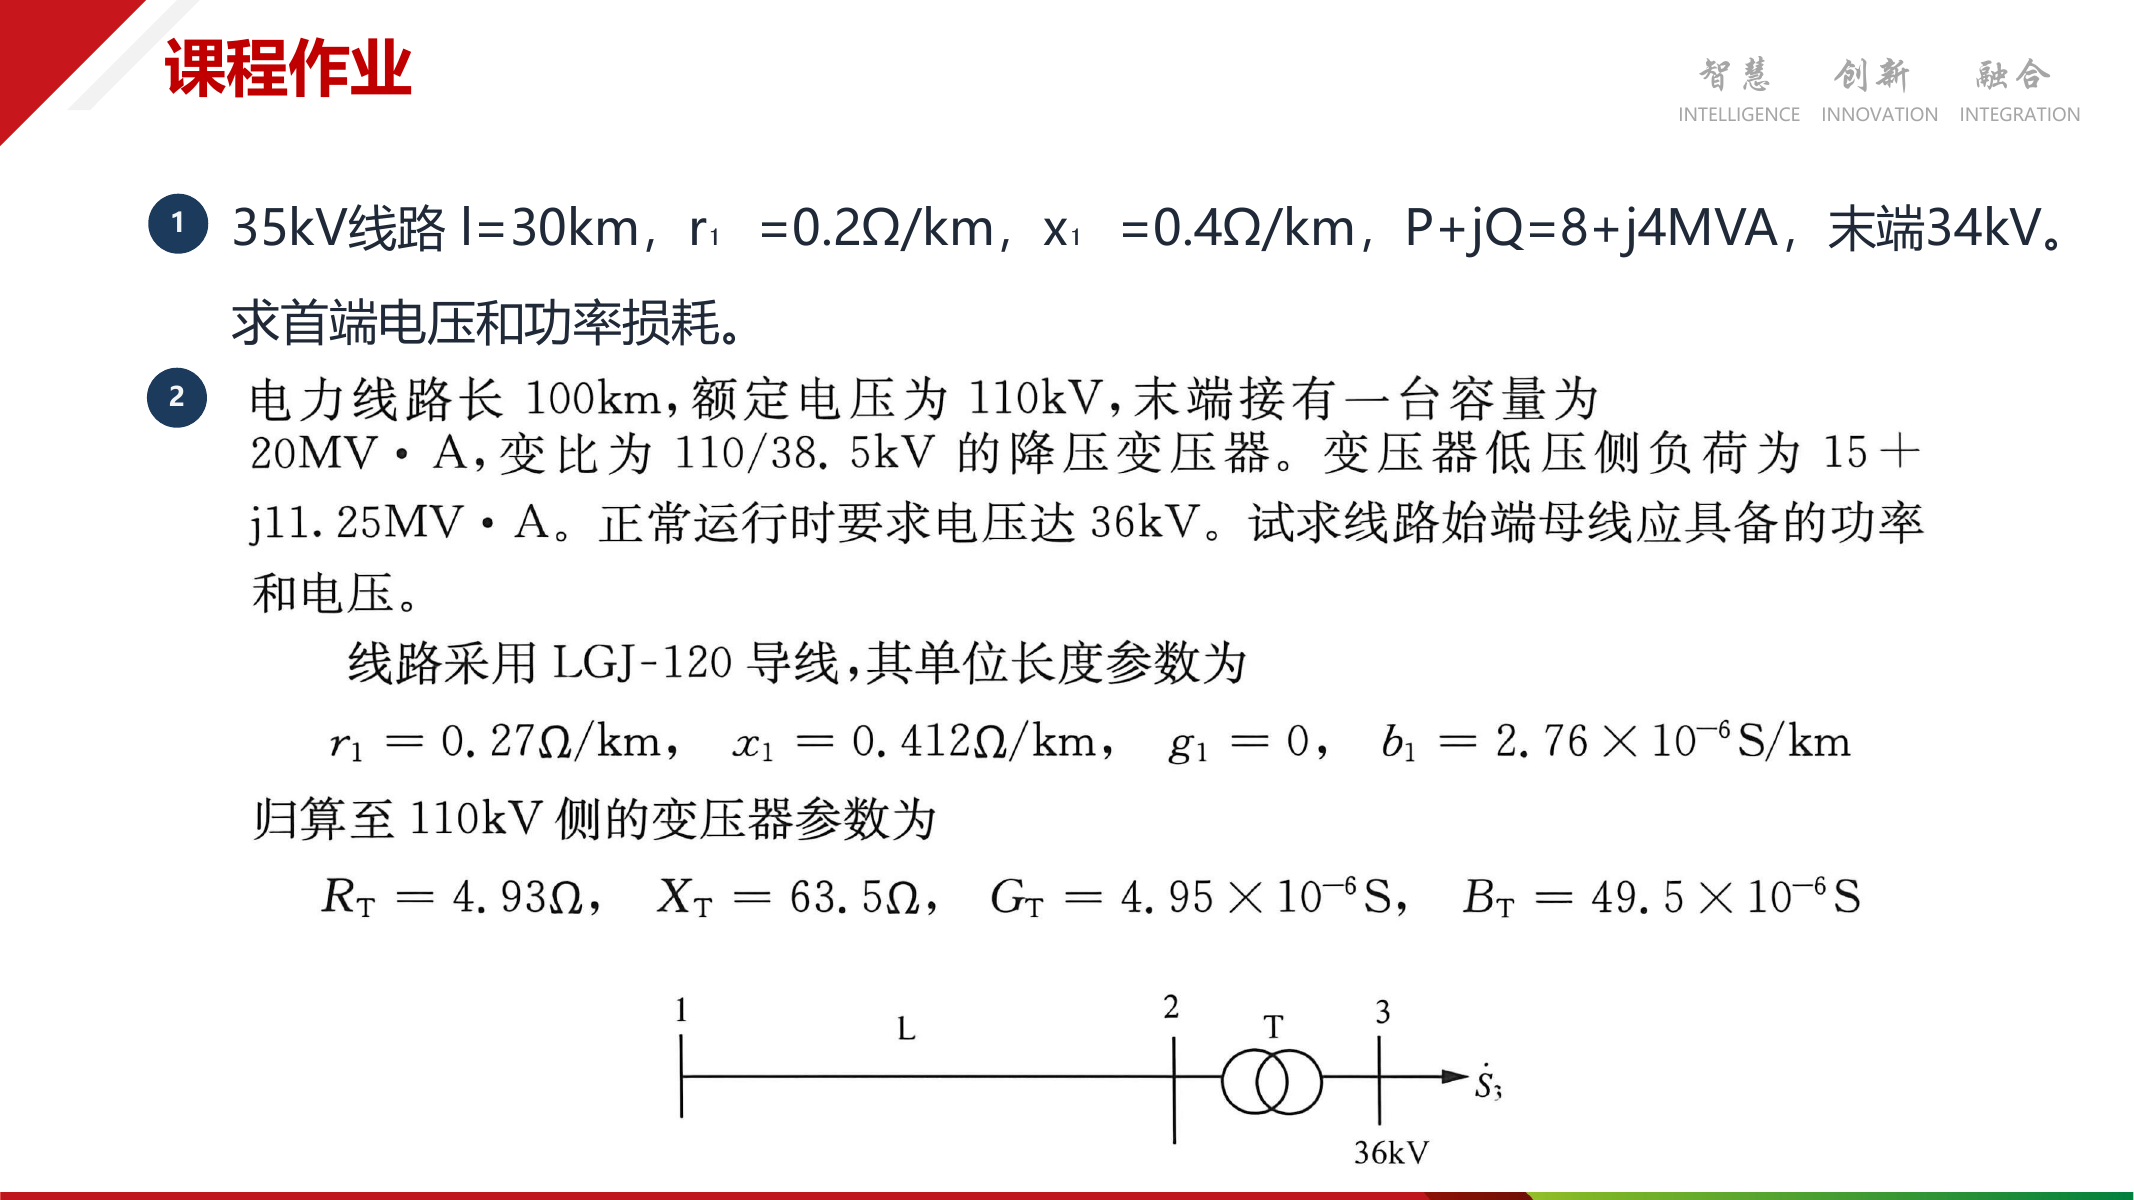
\includegraphics[width=0.96\textwidth]{slide37.png}
    \caption{第八章课件第 37 页：两道作业题原文及第 2 题接线图}
    \label{fig:slide37}
\end{figure}

\begin{figure}[H]
    \centering
    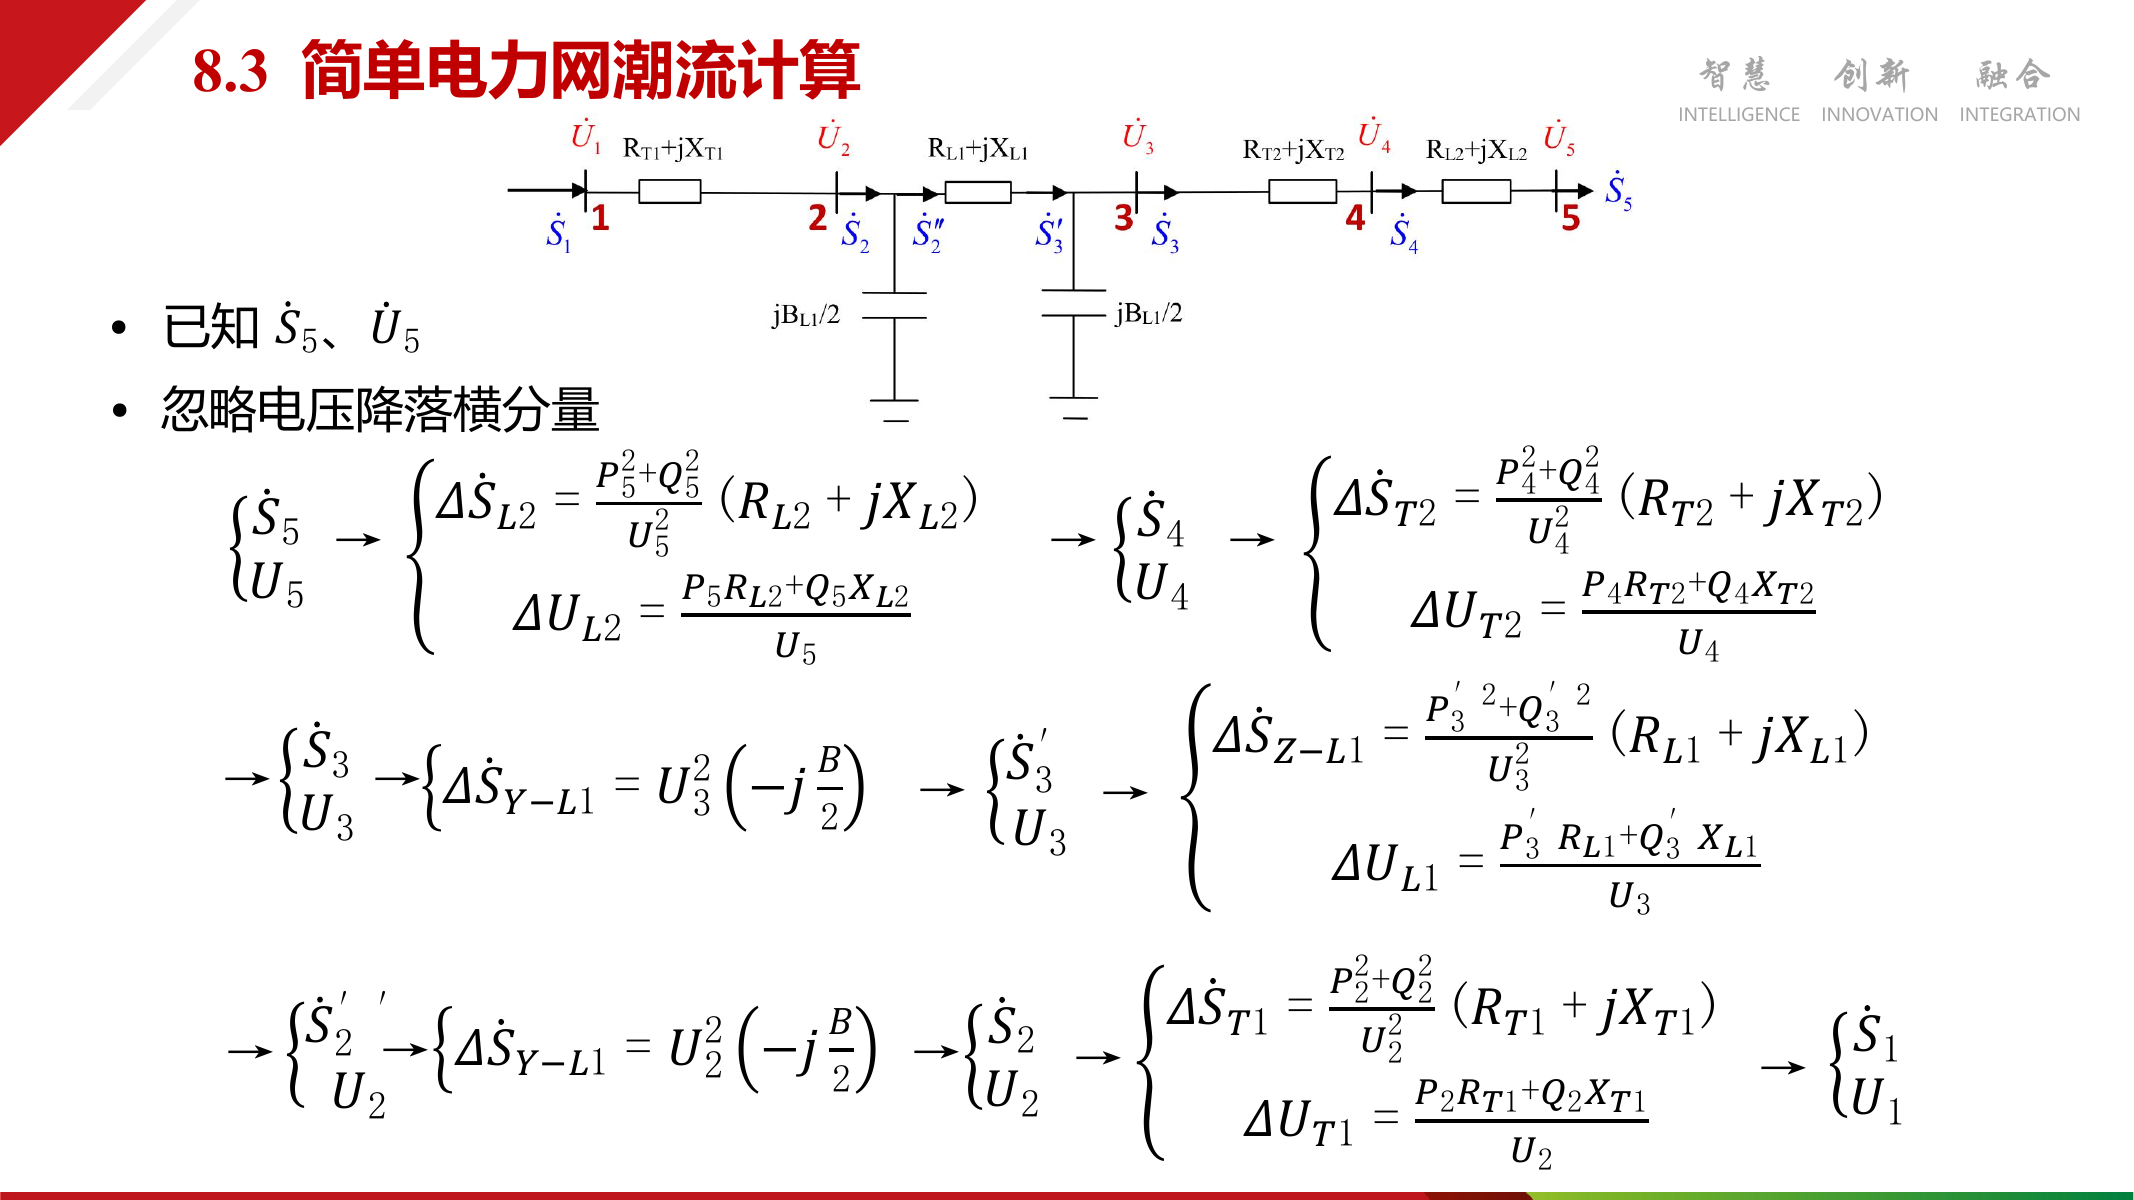
\includegraphics[width=0.96\textwidth]{slide14.png}
    \caption{第八章课件第 14 页：开式网“已知末端功率、电压”的逐段推算法}
    \label{fig:slide14}
\end{figure}
